\documentclass{beamer}
\mode<presentation>
{
  \usetheme{CambridgeUS}
  \usecolortheme{beaver}
  \usefonttheme{professionalfonts}
  \setbeamertemplate{navigation symbols}{}
  \setbeamertemplate{caption}[numbered]
} 

\usepackage{fontspec}
\setmainfont{CMU Serif}[Ligatures=TeX]
\setsansfont{CMU Sans Serif}[Ligatures=TeX]
\usepackage[russian,english]{babel}
\usepackage{subfigure}

\title[RL для промышленных роботов]{Обучения с подкреплением \\для управления промышленным роботом}
\author{Юнес Али}
\institute [МГТУ им. Н.Э. Баумана]{
Группа: СМ7и-43М\\ \vspace{0.5cm}
Руководитель:\\
Ющенко Аркадий Семёнович\\ \vspace{1cm}
Московский государственный технический университет \\ имени Н.Э. Баумана \\ (национальный исследовательский университет)
}
\logo{

\includegraphics[height=3cm]{img/logo.png}
}
\date{}

\begin{document}

\begin{frame}\relax
    \titlepage
\end{frame}
\logo{}
\begin{frame}{Contents}
    \tableofcontents
\end{frame}
\setbeamercovered{transparent}
\section{Введение}
\begin{frame}{Мотивация}
    \begin{itemize}
        \item <1> Классическое управление хорошо работает в структурированных средах, когда у нас есть хорошие модели робота и окружающей среды.
        \item <2> Но, если модель робота неизвестно (или известно неточно ), как можно управлять его?
        \only<2> {
        \\
        На пример, робот который мы собирали и использовали для диплома в бакалавре \\
        (Тишренский университет, Сирия - 2017)\\
        \begin{figure}
            \centering
            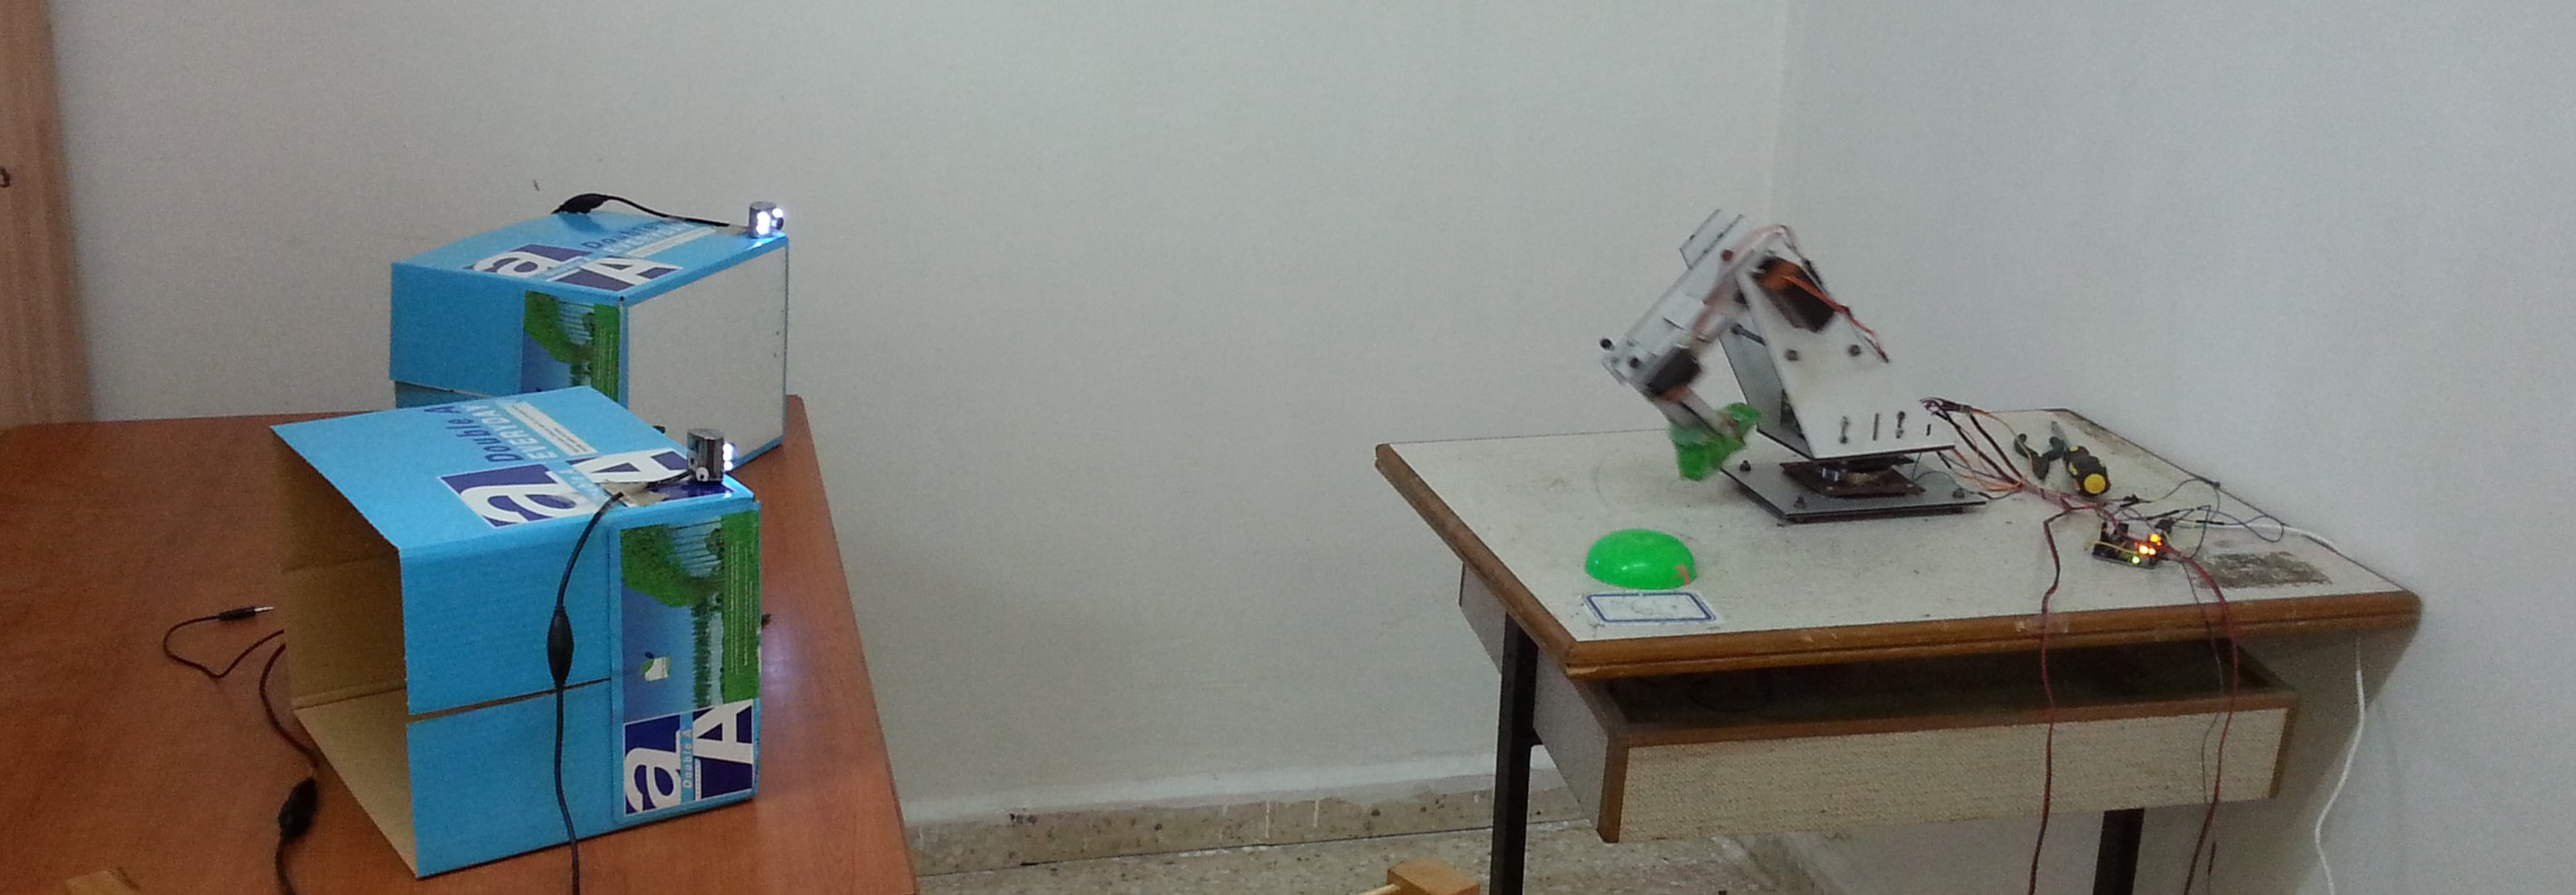
\includegraphics[width=0.86\textwidth]{img/grad1.jpg}
        \end{figure}
        }
        \item <3> Мы предлагаем использовать обучения с подкреплением для управления промышленных роботов.
        \only<3>{\\
        Обучения с подкреплением зависит от проб и ошибок.
        \begin{figure}
            \centering
            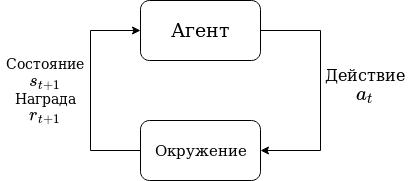
\includegraphics[width=0.7\textwidth]{img/RL_ru.png}
        \end{figure}
        }
        \item <4> Цель состоит в исследования алгоритмов позволяющих автоматическое проектирование робототехнических систем, с минимальным усилием проектировщика, и с высокой способностей адаптации на новые задачи.
    \end{itemize}
\end{frame}
\begin{frame}{Актуальность и новизна}
    \begin{itemize}
        \item <1-4> Управление на основе обучения поможет в промышленных приложений;
        \only <2-4>{
        \begin{enumerate}
            \item <2> Позволит уменьшить инженерные усилия по установке робота в новых условиях и при решении новых задач.
            \item <3> В случае малых и средних производств.
            \item <4> Облегчит использование недорогих роботов в промышленности.
        \end{enumerate}}
        \item <5-7> Управление на основе обучения важен не только для промышленных манипуляторов, но также для других типов;
        \only<6-7>{
        \begin{enumerate}
            \item <6> Для манипуляторов, кинематика которых известна неточно, например, космических.
            \item <7> Для манипуляторов с избыточностью.
        \end{enumerate}}
        \item <8-10> Сначала, мы исследовали современные алгоритмы обучения с подкреплением, новизна состоит в:
        \begin{enumerate}
            \item <9> Предложение лучший алгоритм обучения с подкреплением для управления промышленных роботов, на основе результаты исследования.
            \item <10> Предложение вспомогательной системой обучения представлению, позволяет настройка поильного система в соответствии с нашим цели.
        \end{enumerate}
    \end{itemize}
\end{frame}
\begin{frame}{Задача}
    \begin{itemize}
        \item <1> Задачей сборки является важнейший часть применения робототехники в промышленности.
        \item <2> Наиболее распространенной проблемой робототехнической сборки является случай введения стержня в отверстии.
        \item <3-5> Контрольные примеры в нашем проекте:
        \begin{enumerate}
            \item <4> Захват куба и вставка его в отверстие
            \item <5> Вставка электрического разъема USB
        \end{enumerate}
        \only<4>{
        \begin{figure}[H]
    \centering
    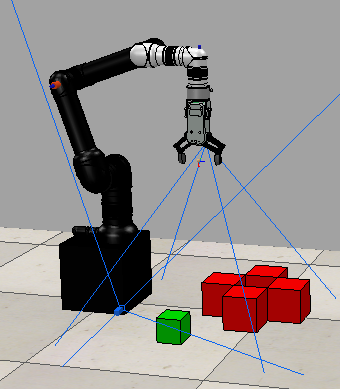
\includegraphics[width=0.27\textwidth]{img/op1.png}
    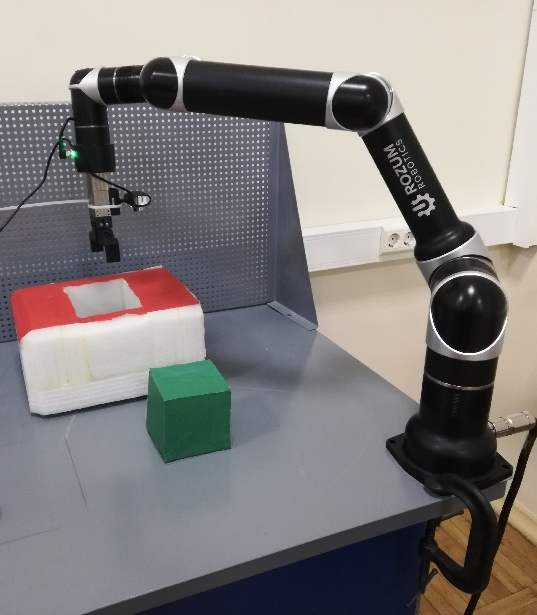
\includegraphics[width=0.27\textwidth]{img/op2.png}
\end{figure}}
\only<5>{
\begin{figure}[H]
    \centering
    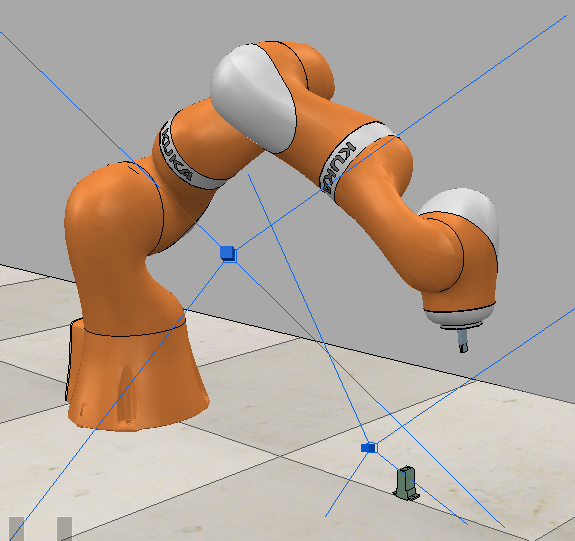
\includegraphics[width=0.27\textwidth]{img/kuka_usb.png}
    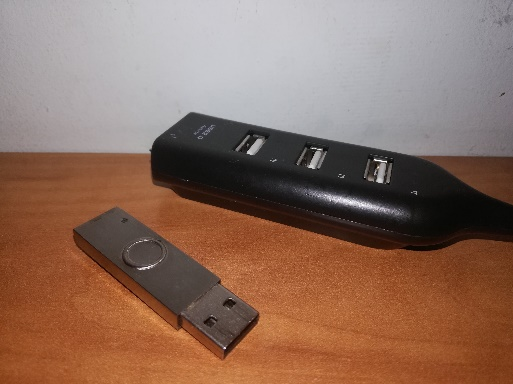
\includegraphics[width=0.3\textwidth]{img/usb.png}
\end{figure}}
    \end{itemize}
\end{frame}

\section{Исследовательская часть}
\begin{frame}{Безмодельное обучение с подкреплением}
    \begin{itemize}
        \item <1> Обучаются непосредственное связи между состояниями (признаки из изображении) и командами управления двигателями.
        \item <2> Мы исследовали алгоритма Soft-Actor Critic (SAC).
        \item <3> Проектировали окружения как Марковский процесс принятии решения, написали и запускали алгоритма в симуляторе.
        \only<3>{
        \begin{figure}
            \centering
            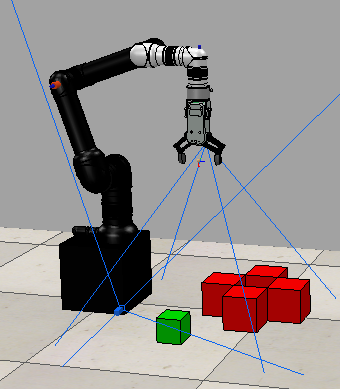
\includegraphics[width=0.35\textwidth]{img/op1.png}
        \end{figure}}
        \item <4> По результатам эксперимента, недостатком этого типа алгоритмов является долгое время обучения (2 дня на сервере).
        \only<4> {
        \begin{figure}
            \centering
            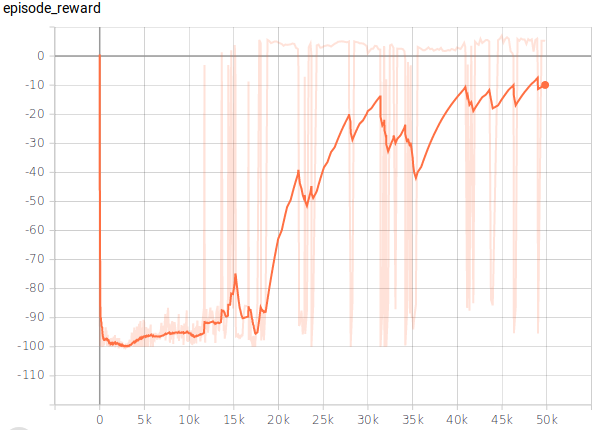
\includegraphics[width=0.45\textwidth]{img/rew.png}
        \end{figure}
        }
        \item <5> Долгое время обучения $\rightarrow$ непрактично для реальных роботов.
    \end{itemize}
\end{frame}
\begin{frame}{Гауссовский процессы и Обучения с подкреплением на основе модели}
    \begin{itemize}
        \item <1> Обучение с подкреплением на основе модели, с Гауссовским процессором в качестве модели.\\
        PILCO: самый эффективный RL алгоритм.\\
        \only<1>{
        x- состояние и u управление.\\
        Обработает неопределенности во входных данных и модели,\\
        Это что нужно для робототехнических систем в практики. 
        \begin{figure}
            \centering
            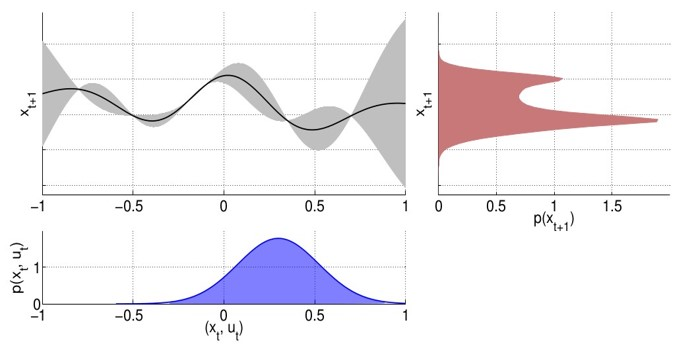
\includegraphics[width=0.6\textwidth]{img/gp.jpg}
        \end{figure}
        }
        \item <2> Мы использовали Гауссовские процессы с RL, тестировали с манипулятором, публиковали 2 статей по результатам работы.\\
        \only<2>{
        Обратной кинематики манипулятора обучается через 4 итерации (50 секунд на робот) 
        \begin{figure}
            \centering
            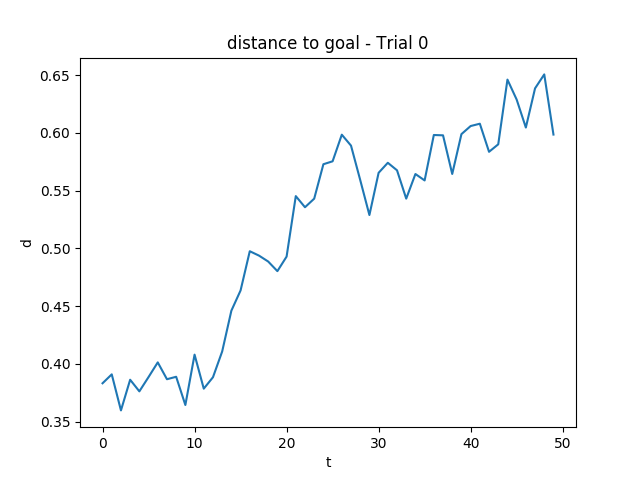
\includegraphics[width=0.225\textwidth]{img/dist0.png}
            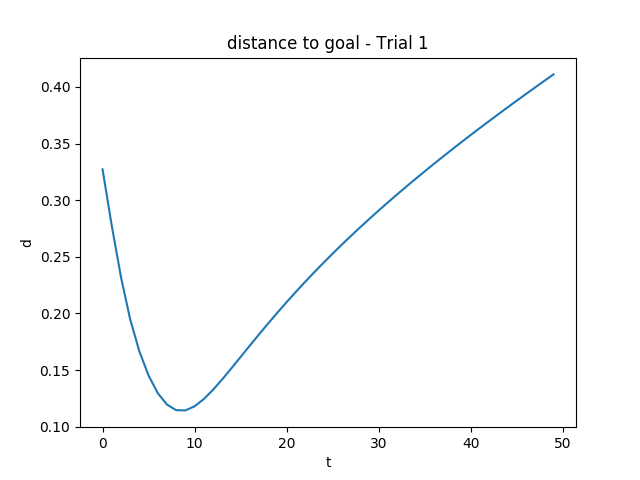
\includegraphics[width=0.225\textwidth]{img/dist1.png}
            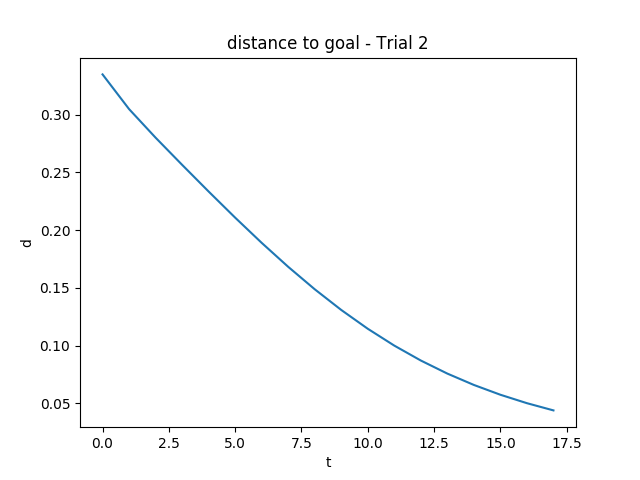
\includegraphics[width=0.225\textwidth]{img/dist2.png}
            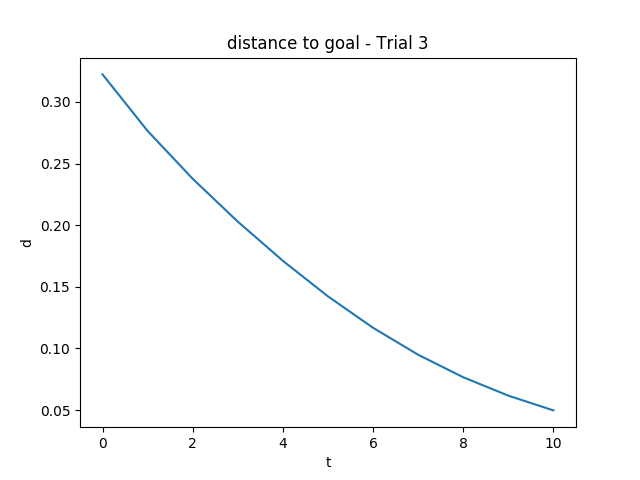
\includegraphics[width=0.225\textwidth]{img/dist3.png}
        \end{figure}
        }
        \item <3> Недостаток PILCO, работает только с дифференцируемые функции стоимости, и с высокой вычислительной сложностью.
    \end{itemize}
\end{frame}
\begin{frame}{Предложенный метод}
\begin{itemize}
    \item <1> Нам нужно компромисс между безмодельными алгоритмами, и алгоритмами типа PILCO. 
    \item <2> Ансамбль нейронных сетей (ENN) является заменой гауссовских процессов с низкой вычислительной сложностью.
    \only<2>{
    \begin{figure}
        \centering
        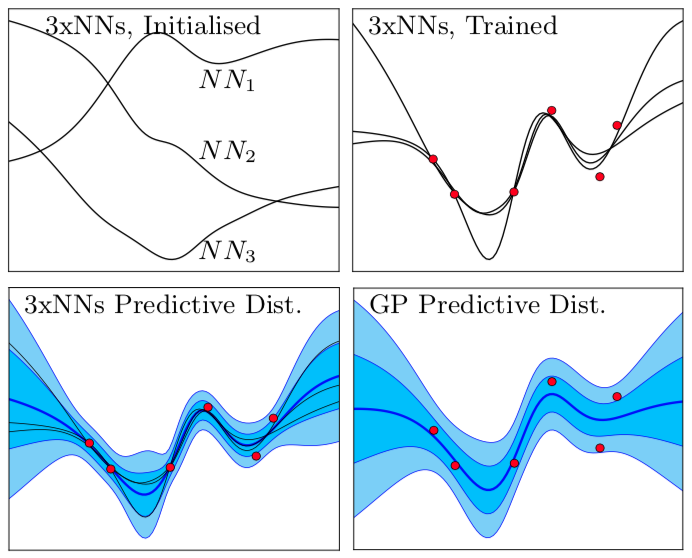
\includegraphics[width=0.5\textwidth]{img/ensemble_intro.png}
    \end{figure}
    }
    \item <3> Мы решили проблему по использованию ансамбль нейронных сетей в качестве модели для обучения с подкреплением.
    \only <3>{
    \begin{figure}
        \centering
        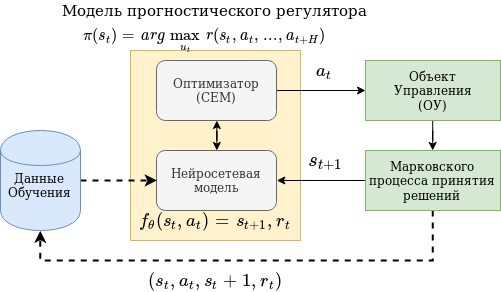
\includegraphics[width=0.5\textwidth]{img/MPC_ru.png}
    \end{figure}
    }
    \item <4> Алгоритм можно рассматривать как модельное прогнозирующее управление на основе обучения.
    \item <5> мы разработали целый фреймворк с экспериментами на промышленном манипуляторе.
\end{itemize}
    
\end{frame}
\section{экспериментальная часть}
\begin{frame}{Эксперименты - в симуляторе}
    \begin{itemize}
        \item <1> Состояния и вычисления стоимости зависит от места положения объектов в рабочим зоне.
        \item <2-6> Моделирование операции захват куба и вставление его в отверстие.
        \only <2>{\\
        Модель переходности
        \begin{figure}
            \centering
            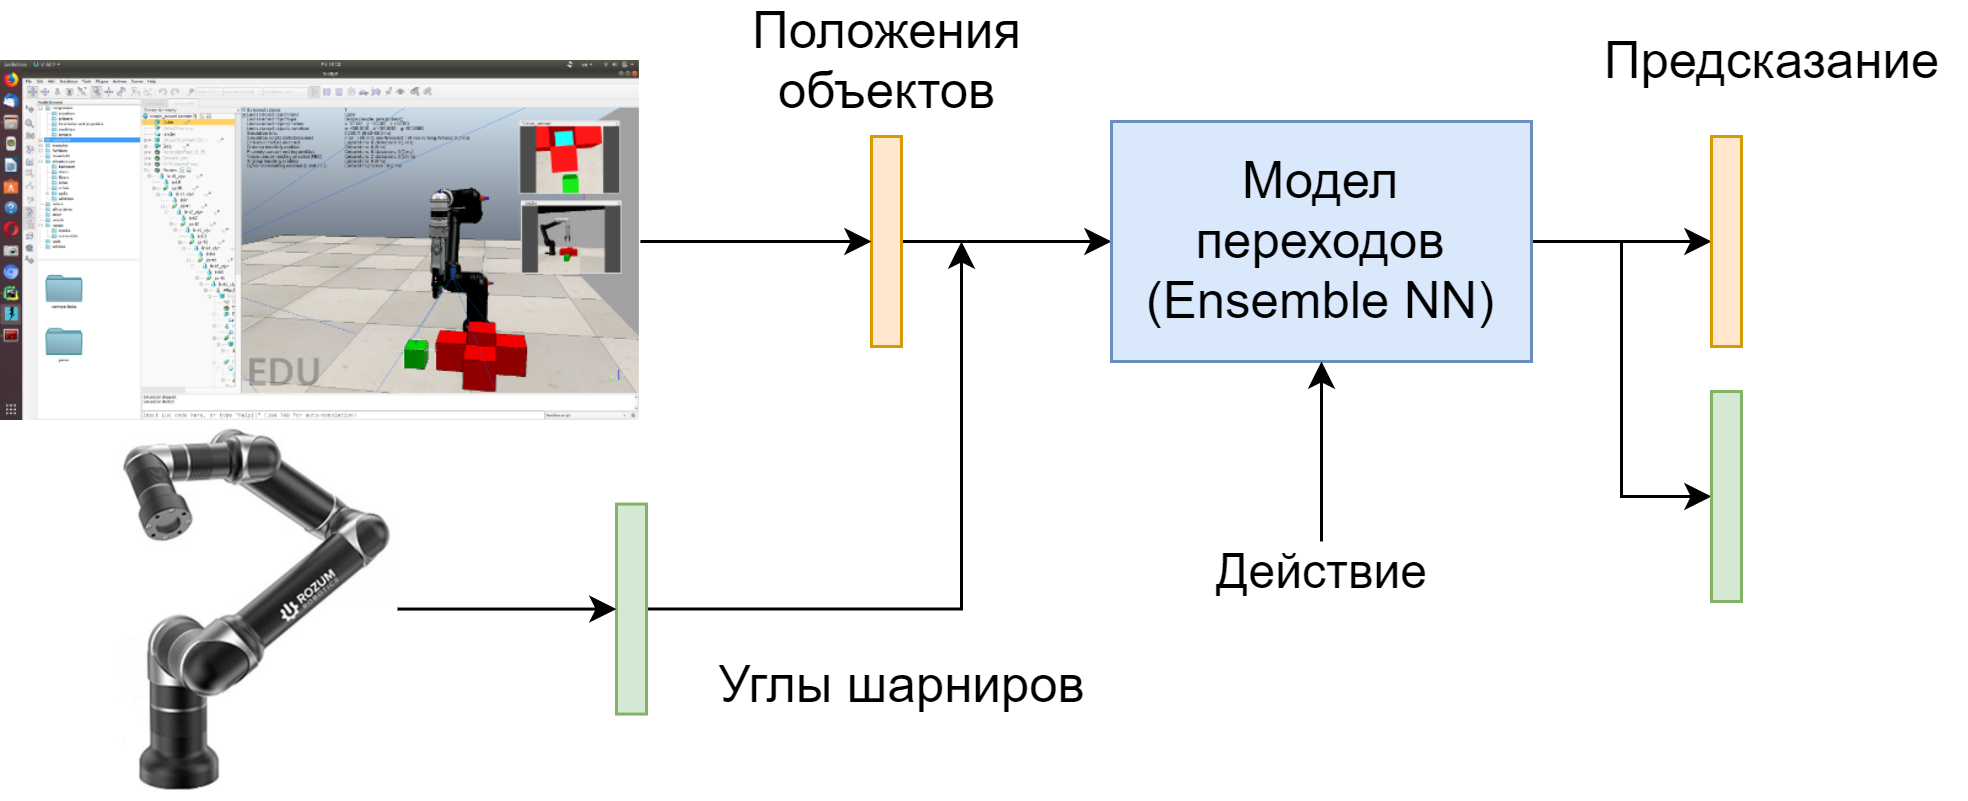
\includegraphics[width=0.8\textwidth]{img/dia1.png}
        \end{figure}
        }
        \only <3>{\\
        Корректировка реакцию на ступеньку за время обучения - Итерация № 0
        \begin{figure}
            \centering
            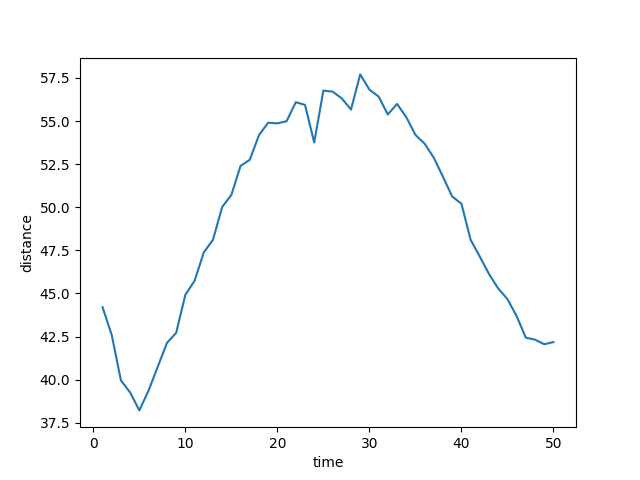
\includegraphics[width=0.55\textwidth]{img/step_response0.png}
        \end{figure}
        }
        \only <4>{\\
        Корректировка реакцию на ступеньку за время обучения - Итерация № 5
        \begin{figure}
            \centering
            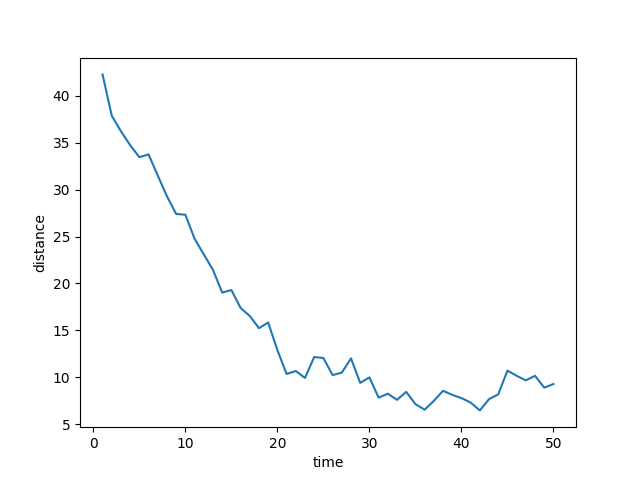
\includegraphics[width=0.55\textwidth]{img/step_response5.png}
        \end{figure}
        }
        \only <5>{\\
        Корректировка реакцию на ступеньку за время обучения - Итерация № 8
        \begin{figure}
            \centering
            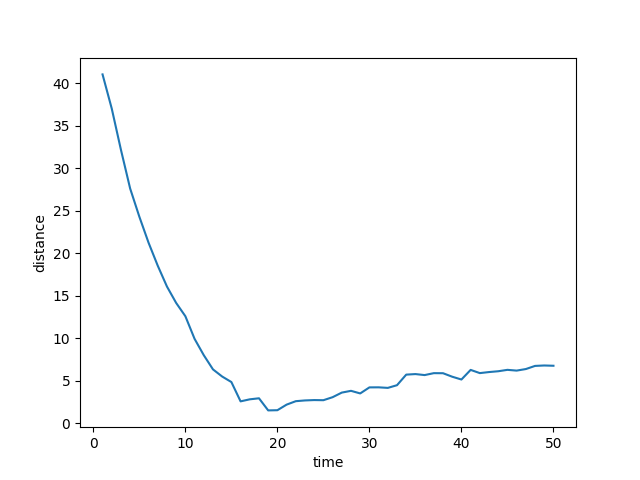
\includegraphics[width=0.55\textwidth]{img/step_response8.png}
        \end{figure}
        }
        \only <6>{\\
        Реакция обученнной системы на ступеньку - Итерация № 50
        \begin{figure}
            \centering
            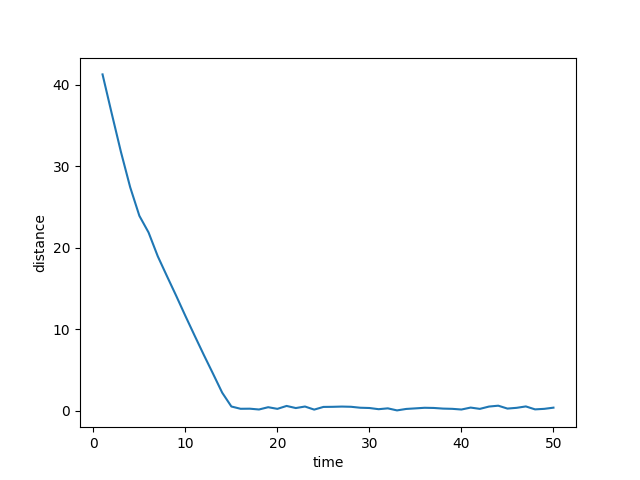
\includegraphics[width=0.55\textwidth]{img/step_response49.png}
        \end{figure}
        }
        \item <7-8> Моделирование задачи по вставке электрического разъема USB с помощью  манипулятора.
        \only <7>{
        \\
        Модель переходности
        \begin{figure}
            \centering
            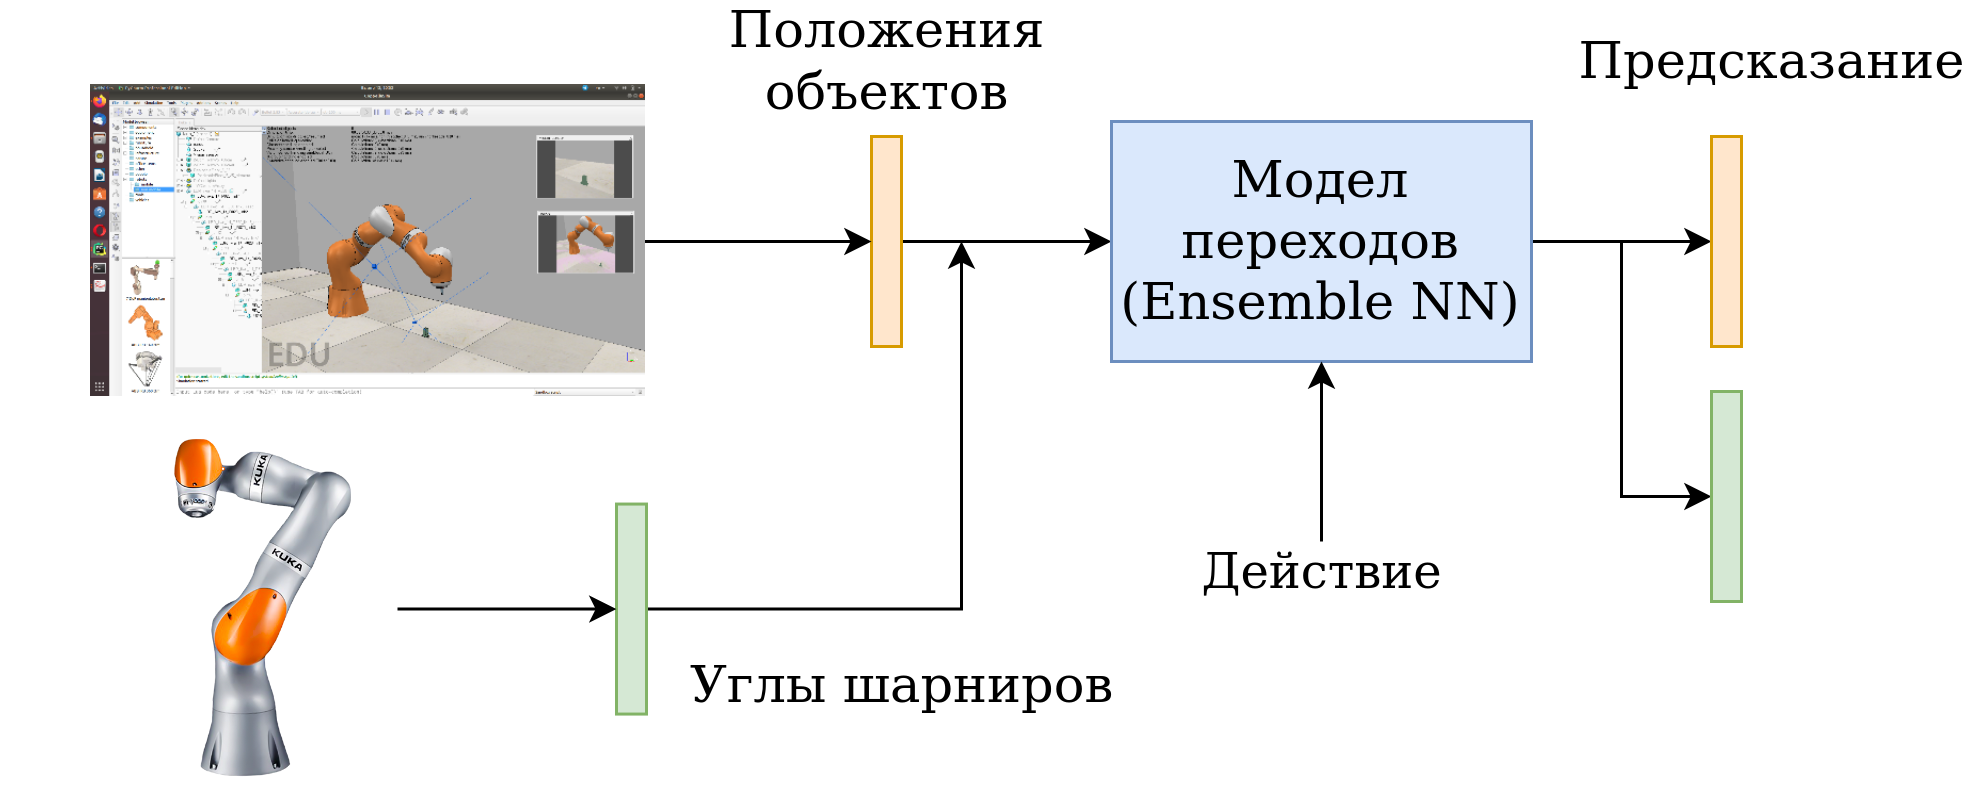
\includegraphics[width=0.8\textwidth]{img/dia3.png}
        \end{figure}
        }
        \only <8>{
        \\
        График изменения величины вознаграждения в задаче вставки USB - чем больше, тем лучше
        \begin{figure}
            \centering
            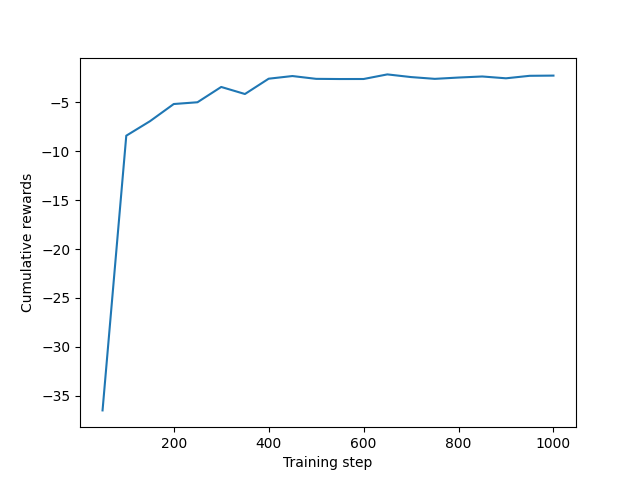
\includegraphics[width=0.5\textwidth]{img/usb_bbest_50_rewards.png}
        \end{figure}
        }
    \end{itemize}
\end{frame}

\begin{frame}{Эксперименты - в реальном мире}
    \begin{itemize}
        \item  <1> Состояния и вычисления стоимости зависит по использованию данных из сенсоров (RGB изображений).
        \item <2-3> Захват куба и вставление его в отверстие с помощью реального манипулятора.
        \only <2>{\\
        Модель переходности - СТЗ зависит от цвета
        \begin{figure}
            \centering
            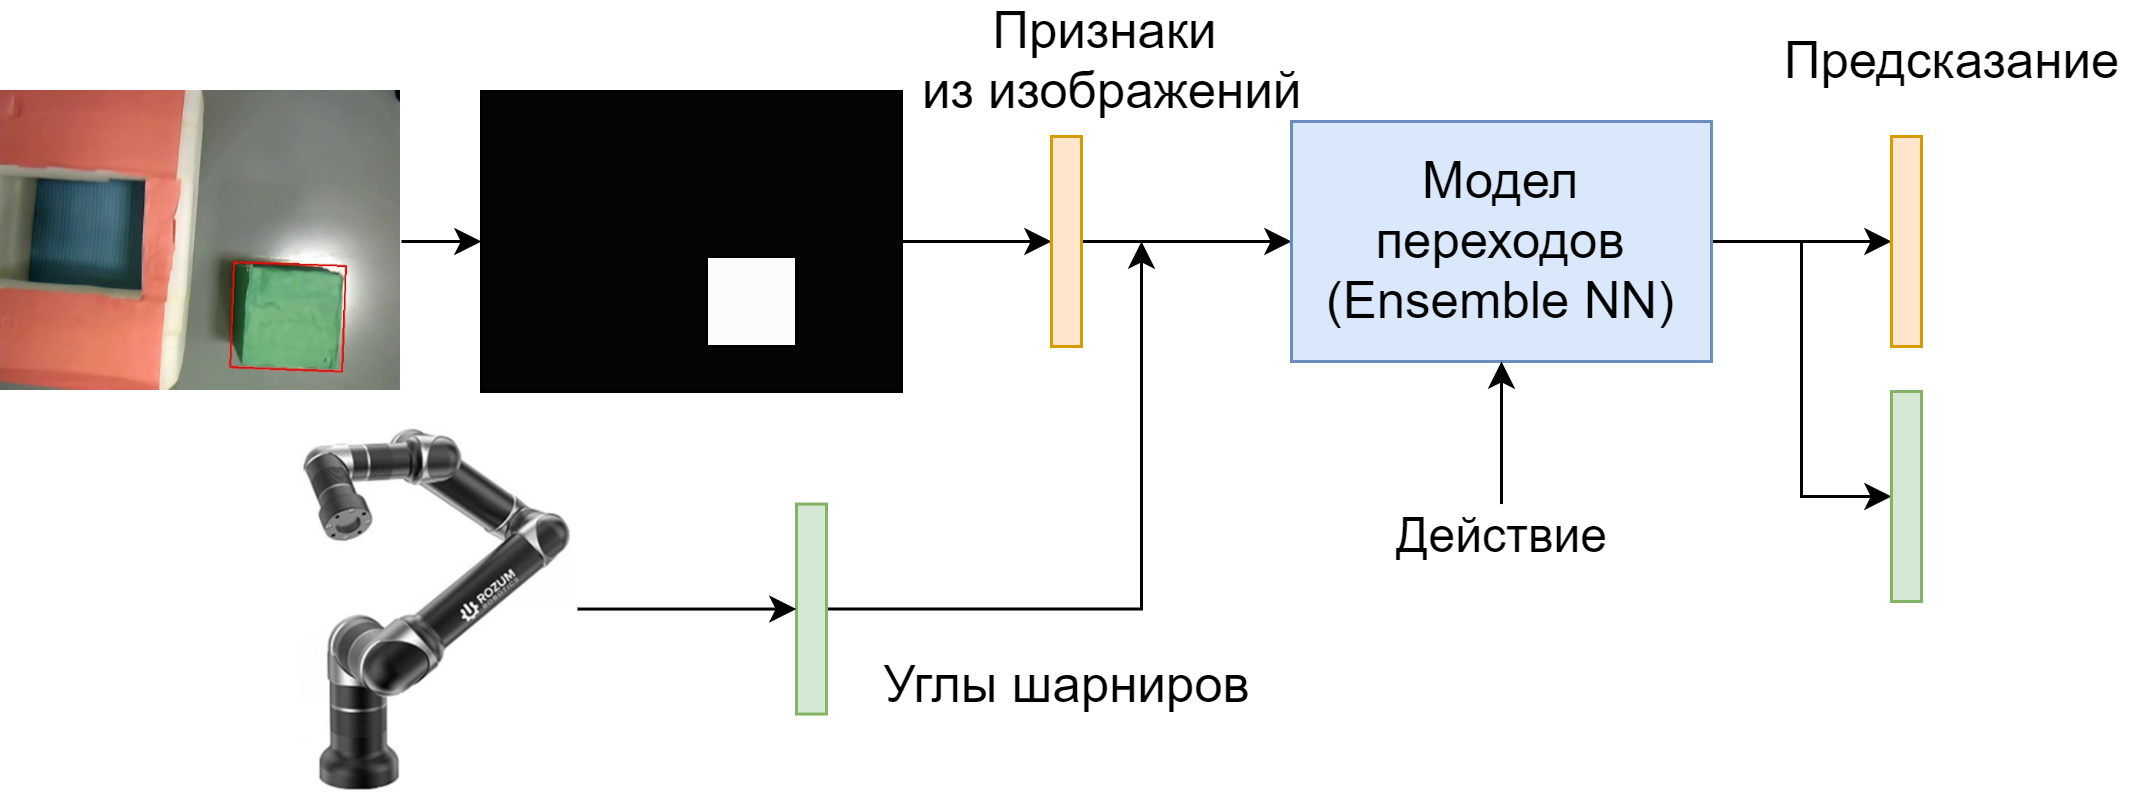
\includegraphics[width=0.8\textwidth]{img/dia2.png}
        \end{figure}
        }
        \only <3>{
        \\
        График изменения вознаграждения в процессе обучения реального робота- чем больше, тем лучше
        \begin{figure}
            \centering
            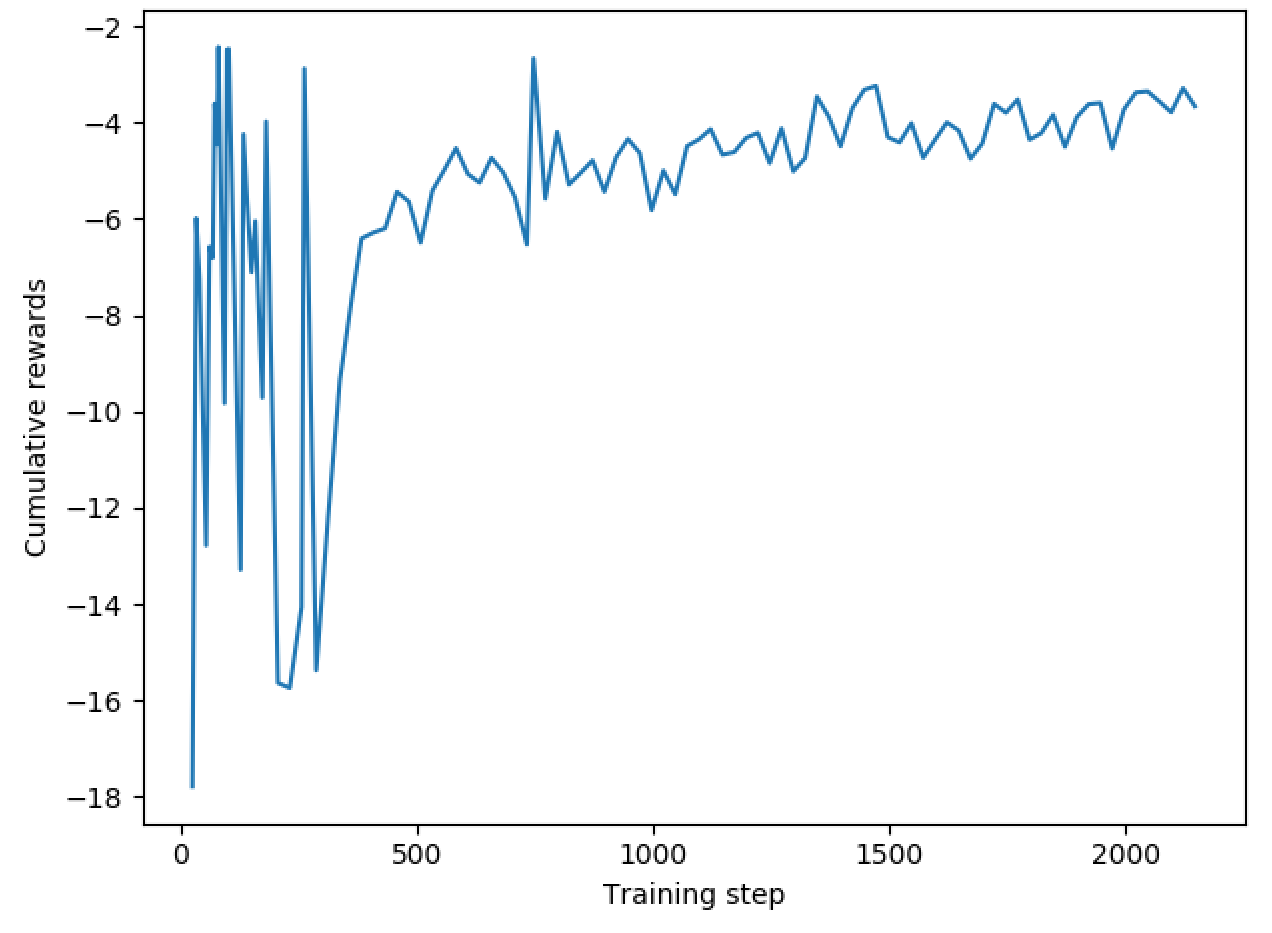
\includegraphics[width=0.55\textwidth]{img/real_rozum_rew.png}
        \end{figure}
        }
        \item <4-7> Вставка электрического разъема USB с помощью  реального манипулятора
        \only <4>{\\
        Модель переходности - Систем обучения представлению
        \begin{figure}
            \centering
            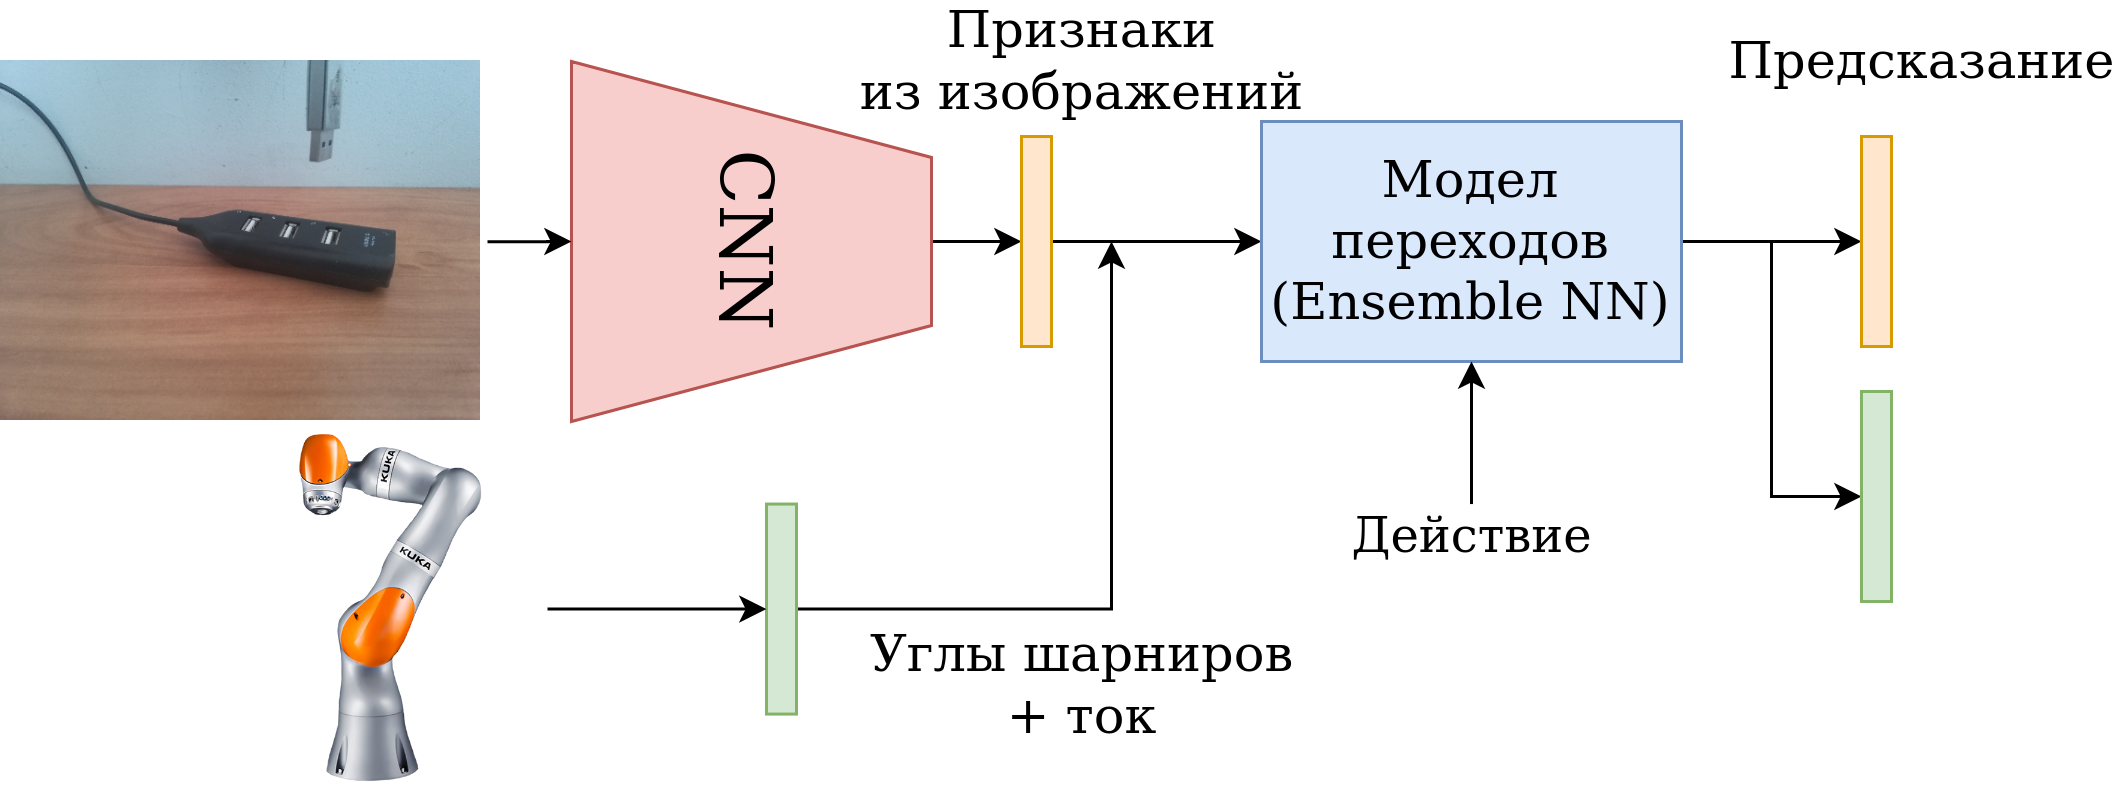
\includegraphics[width=0.8\textwidth]{img/dia4(1).png}
        \end{figure}
        }
        \only <5>{\\
        Архитектура обучения модели вложения - вектор в латентном пространстве для каждого изображения
        \begin{figure}
            \centering
            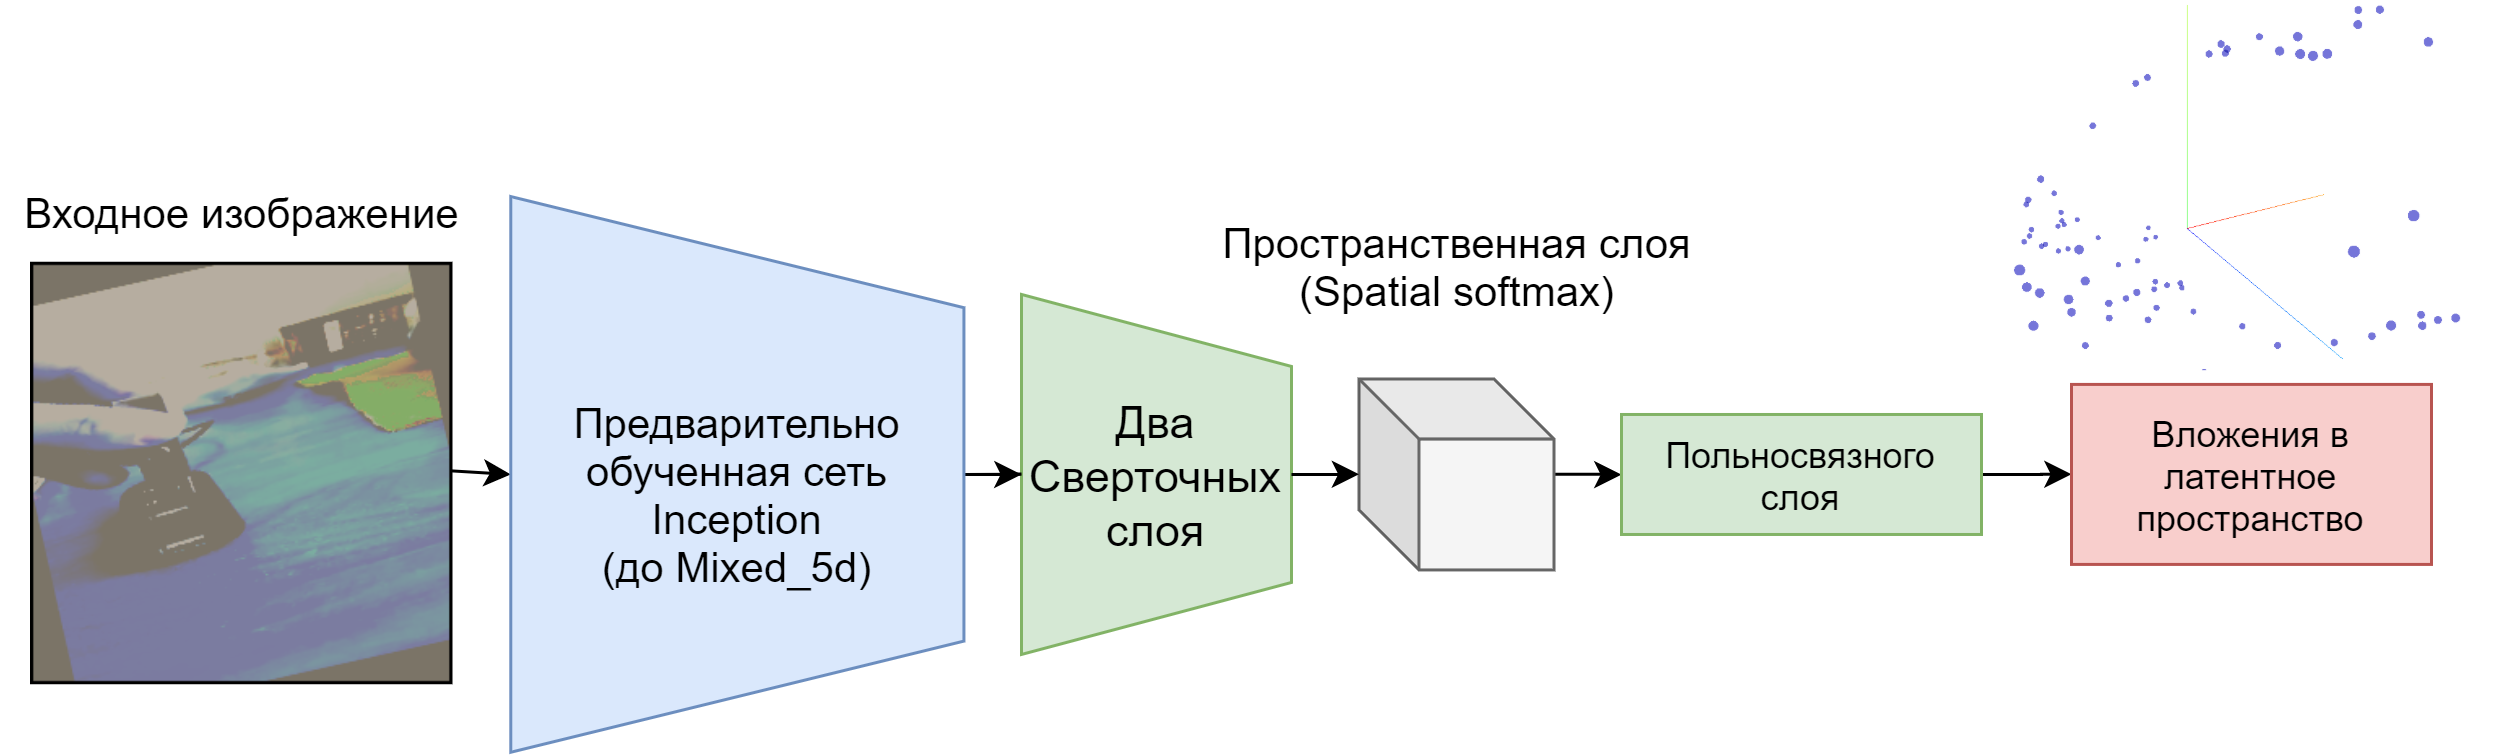
\includegraphics[width=0.8\textwidth]{img/SCL_ru.png}
        \end{figure}
        }
        \only <6>{\\
        Латентное пространство и вознаграждение перед запуском обучения - вознаграждения  зависит от расстояния до целевого изображения в Латентном пространстве
        \begin{figure}
            \centering
            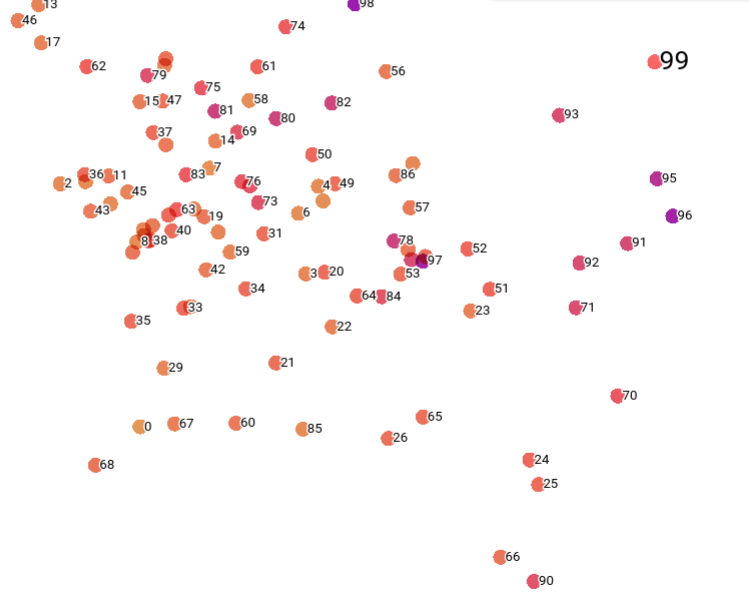
\includegraphics[width=0.3\textwidth]{img/latent0.png}
            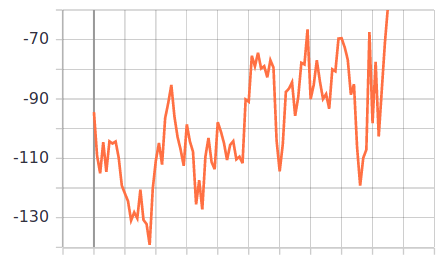
\includegraphics[width=0.4\textwidth]{img/cost0.png}
        \end{figure}
        }
        \only <7>{\\
        Латентное пространство и вознаграждение после обучения - вознаграждения  зависит от расстояния до целевого изображения в Латентном пространстве
        \begin{figure}
            \centering
            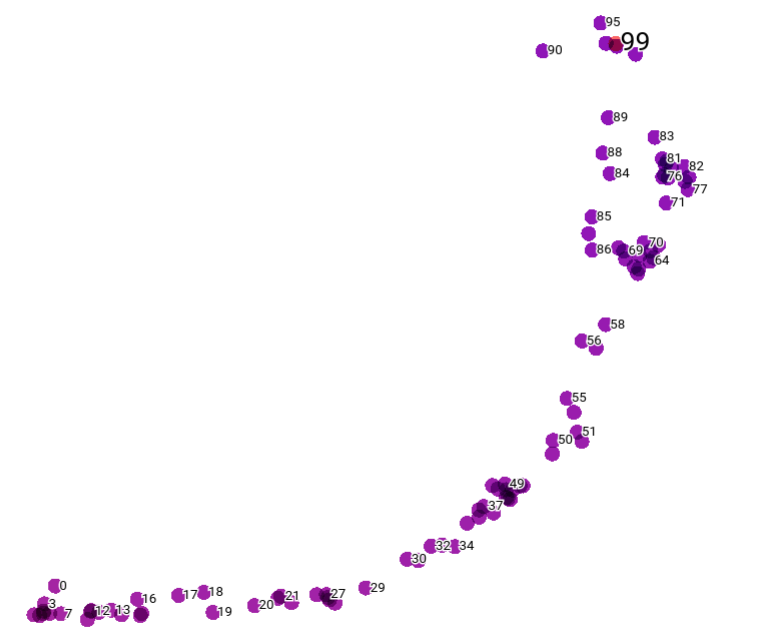
\includegraphics[width=0.3\textwidth]{img/latent10000.png}
            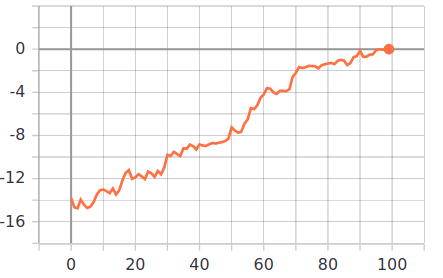
\includegraphics[width=0.4\textwidth]{img/cost20.png}
        \end{figure}
        }
        \only <8-9>{
        \item <8> Мы предлагали систему обучения без учителя, которая позволяет формировать представления состояний для робототехниких задач. Алгоритм требует только несколько видеороликов, демонстрирующих необходимую задачу.
        \item <9> Мы называли алгоритма последовательное контрастивное обучение (SCL), провели экспериментов и публиковали статью.
        }
    \end{itemize}
\end{frame}
\section{Заключения}
\begin{frame}{Выводы}
\begin{itemize}
    \item <1> Использование обучения в робототехнических системах имеет перспективный будущий. Но нам нужно работать на разработки эффективные алгоритмы, мы работали с обучением с подкреплением и обучение без учителя.
    \item <2> Мы предлагали алгоритм обучения с подкреплением, позволяет эффективно обучать робот задачу через 5-10 минут на реальном роботе (всего обучения 30-45 минут).
    \item <3> Мы предлагали алгоритм обучении представлению, позволяет обучать представление из видеороликов (даже со смартфона).
    \item <4> Предлагаемые алгоритмы обучения с подкреплением и обучения представлению формируют поильный фреймворк для обучения роботов с минимальным усилием проектировщика.
\end{itemize}
\end{frame}
\begin{frame}{Исследовательские деятельности}
\begin{itemize}
    \item Volunteer at ICRA and ICLR conferences 2020.
    \item Reviewer at IROS- RAL IEEE conference 2020
    \item Full scholarship to Machine learning summer school London 2019
    \item Full scholarship to ETHz robotic summer scholl Zurich 2019
    \item 2 статьи – Scopus:\\
    Younes, A., & Yushchenko, A. S. (2019, November). Toward faster reinforcement learning for robotics applications by using Gaussian processes. In AIP Conference Proceedings (Vol. 2171, No. 1, p. 190007). AIP Publishing LLC.\\
    Younes, A., & Panov, A. I. (2019). Toward Faster Reinforcement Learning for Robotics: Using Gaussian Processes. In Artificial Intelligence (pp. 160-174). Springer, Cham.
    \item 1 статья в публикации:\\
    Ali Younes and Aleksandr I. Panov: Sequential Contrastive Learning to Master Effective Representations for Reinforcement Learning and Control, submitted.
\end{itemize}
\end{frame}
\end{document}